
\begin{Schunk}
\begin{Sinput}
> library(knitr)
> options(warn=-1)
> opts_chunk$set(
+ fig.path='fig/tartu-', tidy=FALSE, fig.height=4, size="scriptsize"
+ )
\end{Sinput}
\end{Schunk}

\def\R{\texttt{R}}
\def\pkg#1{{\bf #1}}

% \section{Outline}
% \label{sec:xxx}


%% \section{History}
%% \label{sec:history}

%% \begin{sframe}
%% \frametitle{Some history}
%%   \begin{itemize}
%%   \item Years ago, Ulrich Halekoh and SH colleagues at ``Danish Institute for Agricultural Sciences''
%%   \item That was SAS-country back then
%%   \item Many studies called for random effects models - and for \texttt{PROC MIXED}
%%   \item \texttt{PROC MIXED} reports (by default) $p$--values from asymptotic likelihood ratio test. 
%%   \item Main concern: Effects should be ``tested against'' the correct variance
%%     component in order not to make effects appear more significant than they
%%     really are.
%%   \end{itemize}
%% \end{sframe}

%% \begin{sframe}
%% \frametitle{Then \R\ came along...}
%% \begin{itemize}
%%   \item Common advice: Use Satterthwaite or Kenward-Roger approximation of denominator
%%     degrees of freedom in $F$-test -- in an attempt not to get things ``too wrong''.
%% \item Then \R\ came along; we advocated the use of \R.  
%% \item Random effects models were fitted with the \pkg{nlme} package -- but there
%%   was no Satterthwaite or Kenward-Roger approximation, so our common advice fell
%%   apart.
%% \end{itemize}
%% \end{sframe}

%% \subsection{The degree of freedom police...	}
%% \label{sec:degr-freed-polic}

%% \begin{sframe}{asdasd}
%% \frametitle{The degree of freedom police}

%% R-help - 2006: \texttt{[R] how calculation degrees freedom}

%% \url{https://stat.ethz.ch/pipermail/r-help/2006-January/087013.html}

%% SH: Along similar lines ...  probably in recognition of the degree of freedom problem. It could be nice, however, if anova() produced ... 

%% Doug Bates: I don't think the "degrees of freedom police" would find that to be a
%% suitable compromise. :-)

%% In reply to another question:

%% Doug Bates: I will defer to any of the "degrees of freedom police" who post to
%% this list to give you an explanation of why there should be different
%% degrees of freedom. 

%% \end{sframe}


\section{Outline}
\label{sec:outline}


\section{A small example}
\label{sec:small}

\begin{frame}
  {here,kkk}

  
  Very simple setup: One-way-anova: Compare treatment with a control; 5
units (persons, animals...) per group; each unit is measured
twice. Measurements on same unit are positively correlated.

Problem: If we ignore  clustering/positive correlation:
\begin{itemize}
\item pretending to have
  more information than we have
  
\item standard errors of estimates become
  too small 
\item effects appear stronger than they really are.
\end{itemize}


\begin{Schunk}
\begin{Sinput}
> dub
\end{Sinput}
\begin{Soutput}
            y1 y2  trt  subj
1   0.70409556  0 ctrl subj1
2   1.00904041  0 ctrl subj1
3  -0.34957137  0 ctrl subj2
4   0.39137237  2 ctrl subj2
5  -0.69128595  1 ctrl subj3
6  -0.06265695  0 ctrl subj3
7  -2.45107333  0 trt1 subj4
8  -1.79713108  2 trt1 subj4
9   1.49399598  4 trt1 subj5
10  1.53085564  5 trt1 subj5
11  0.94005852  2 trt1 subj6
12  1.02325089  0 trt1 subj6
\end{Soutput}
\end{Schunk}



\end{frame}








\subsection{Motivation: Sugar beets - A split--plot experiment}
\label{sec:xxx}

\begin{sframe}
 \begin{itemize}
 \item Model how sugar percentage in sugar beets depends on
   harvest time and sowing time.
 \item Five sowing times ($s$) and two harvesting times ($h$).
 \item Experiment was laid out in three blocks ($b$).
 \end{itemize}

{\tiny
\begin{verbatim}
Experimental plan for sugar beets experiment

Sowing times:
 1: 4/4, 2: 12/4, 3: 21/4, 4: 29/4, 5: 18/5

Harvest times:
 1: 2/10, 2: 21/10

Plot allocation:
      |  Block 1           |  Block 2           |  Block 3           |
      +--------------------|--------------------|--------------------+
Plot  | h1  h1  h1  h1  h1 | h2  h2  h2  h2  h2 | h1  h1  h1  h1  h1 | Harvest time
1-15  | s3  s4  s5  s2  s1 | s3  s2  s4  s5  s1 | s5  s2  s3  s4  s1 | Sowing time
      |--------------------|--------------------|--------------------|
Plot  | h2  h2  h2  h2  h2 | h1  h1  h1  h1  h1 | h2  h2  h2  h2  h2 | Harvest time
16-30 | s2  s1  s5  s4  s3 | s4  s1  s3  s2  s5 | s1  s4  s3  s2  s5 | Sowing time
      +--------------------|--------------------|--------------------+
\end{verbatim}
}
\end{sframe}

\begin{sframe}
\begin{Schunk}
\begin{Sinput}
> data(beets, package='pbkrtest')
> head(beets)
\end{Sinput}
\begin{Soutput}
  harvest  block  sow yield sugpct
1   harv1 block1 sow3 128.0   17.1
2   harv1 block1 sow4 118.0   16.9
3   harv1 block1 sow5  95.0   16.6
4   harv1 block1 sow2 131.0   17.0
5   harv1 block1 sow1 136.5   17.0
6   harv2 block2 sow3 136.5   17.0
\end{Soutput}
\begin{Sinput}
> library(doBy)
> library(lme4)
\end{Sinput}
\end{Schunk}
\end{sframe}

\begin{sframe}

\begin{Schunk}
\begin{Sinput}
> par(mfrow=c(1,2))
> with(beets, interaction.plot(sow, harvest, sugpct))
> with(beets, interaction.plot(sow, harvest, yield))
\end{Sinput}
\end{Schunk}
\end{sframe}


\begin{sframe}

% Let $h$ denote harvest time ($h=1,2$), $b$ denote block
% ($b=1,2,3$) and $s$ denote sowing time ($s=1,\dots,5$). Let $H=2$,
% $B=3$ and $S=5$.

  \begin{itemize}
  \item 
    For simplicity we assume that there is no interaction between sowing
    and harvesting times.

  \item A typical model for such an experiment would be:
    \begin{equation}
      \label{eq:beetsmodel1}
      y_{hbs} = \mu + \alpha_h + \beta_b + \gamma_s + U_{hb} + \epsilon_{hbs},
    \end{equation}
    where $U_{hb} \sim N(0,\omega^2)$ and $\epsilon_{hbs}\sim
    N(0,\sigma^2)$.
    

  \item Notice that $U_{hb}$ describes the random variation
    between whole--plots (within blocks).

  \end{itemize}

\end{sframe}



\begin{sframe}
As the design is balanced we may make F--tests for each of the effects
as:
\begin{Schunk}
\begin{Sinput}
> beets$bh <- with(beets, interaction(block, harvest))
> summary(aov(sugpct ~ block + sow + harvest + 
+                 Error(bh), data=beets))
\end{Sinput}
\begin{Soutput}
Error: bh
          Df  Sum Sq Mean Sq F value Pr(>F)  
block      2 0.03267 0.01633   2.579 0.2794  
harvest    1 0.09633 0.09633  15.211 0.0599 .
Residuals  2 0.01267 0.00633                 
---
Signif. codes:  0 ‘***’ 0.001 ‘**’ 0.01 ‘*’ 0.05 ‘.’ 0.1 ‘ ’ 1

Error: Within
          Df Sum Sq Mean Sq F value   Pr(>F)    
sow        4   1.01  0.2525     101 5.74e-13 ***
Residuals 20   0.05  0.0025                     
---
Signif. codes:  0 ‘***’ 0.001 ‘**’ 0.01 ‘*’ 0.05 ‘.’ 0.1 ‘ ’ 1
\end{Soutput}
\end{Schunk}

Notice: the F--statistics are $F_{1,2}$ for harvest time and $F_{4,20}$ for
sowing time.
\end{sframe}

\begin{sframe}

Using \code{lmer()} from \pkg{lme4} we can
fit the models and test for no effect of sowing and harvest time as follows:


\begin{Schunk}
\begin{Sinput}
> beet.lg <- lmer(sugpct ~ block + sow + harvest + 
+                       (1 | block:harvest), data=beets, REML=FALSE)
> beet.noh <- update(beet.lg, .~. - harvest)
> beet.nos  <- update(beet.lg, .~. - sow)
\end{Sinput}
\end{Schunk}

\end{sframe}

\begin{sff}

The LRT based $p$--values are anti--conservative: the effect
of harvest appears stronger than it is.
\begin{Schunk}
\begin{Sinput}
> anova(beet.lg, beet.nos)  %>% as.data.frame
\end{Sinput}
\begin{Soutput}
         Df     AIC     BIC logLik deviance Chisq Chi Df Pr(>Chisq)
beet.nos  6  -2.795   5.612  7.398    -14.8    NA     NA         NA
beet.lg  10 -79.998 -65.986 49.999   -100.0  85.2      4  1.374e-17
\end{Soutput}
\begin{Sinput}
> anova(beet.lg, beet.noh)  %>% as.data.frame
\end{Sinput}
\begin{Soutput}
         Df    AIC    BIC logLik deviance Chisq Chi Df Pr(>Chisq)
beet.noh  9 -69.08 -56.47  43.54   -87.08    NA     NA         NA
beet.lg  10 -80.00 -65.99  50.00  -100.00 12.91      1  0.0003261
\end{Soutput}
\end{Schunk}
  
\end{sff}


\subsection{Motivation: A random regression problem}
\begin{sframe}
  \frametitle{Random coefficient model}

  The change with age  of the distance between two cranial
distances was
observed for 16 boys and 11 girls
from age 8 until age 14.

\begin{figure}[ht]
 \centering
 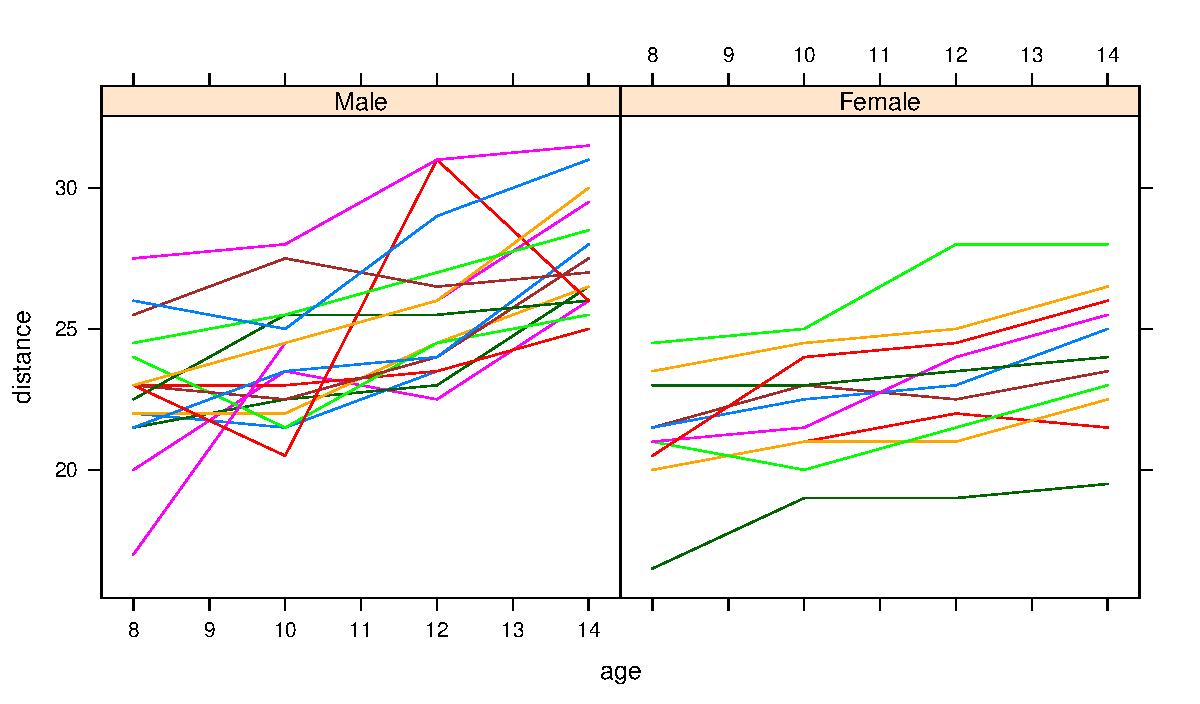
\includegraphics[width=0.7\textwidth]{fig/ortfig01}\\[-0.5cm]
%%\caption{Orthodont data}
 \label{fig:ortfig01}
\end{figure}
\end{sframe}

\begin{sframe}
  \frametitle{Random coefficient model}
  Plot suggests:
\[
dist_{[i]} = \alpha_{sex[i]}
+ \beta_{sex[i]} age_{[i]} + A_{Subj[i]} +
B_{Subj[i]} age_{[i]} + e_{[i]}
\]
with $(A,B) \sim N(0,\bm S)$.

ML-test of $\beta_{boy}=\beta_{girl}$:
\begin{Schunk}
\begin{Sinput}
> ort1ML<- lmer(distance ~ age + Sex + age:Sex + (1 + age | Subject),
+                   REML = FALSE, data=Orthodont)
> ort2ML<- update(ort1ML, .~. - age:Sex)
> as.data.frame(anova(ort1ML, ort2ML))
\end{Sinput}
\begin{Soutput}
       Df   AIC   BIC logLik deviance Chisq Chi Df Pr(>Chisq)
ort2ML  7 446.8 465.6 -216.4    432.8    NA     NA         NA
ort1ML  8 443.8 465.3 -213.9    427.8 5.029      1    0.02492
\end{Soutput}
\end{Schunk}
\end{sframe}


\subsection{Our contribtion}
\label{sec:packages-we-need}



\subsection{Our goal}
\label{sec:our-goal}

\begin{sframe}
\frametitle{Our goal...}
Our goal is to extend the tests provided by \lmer.

There are two issues here:

\begin{itemize}
\item  The choice of test statistic and
  
\item  The reference distribution in which the test statistic is evaluated.
  
\end{itemize}

Implement Kenward-Roger approximation.

Implement parametric bootstrap.

Implement Satterthwaite approximation (not yet released)

\end{sframe}




\section{The Kenward--Roger approach}

\subsection{The Kenward--Roger modification of the $F$--statistic}

\def\transp{^{\top}}
\def\inv{^{-1}}


\begin{sframe}
\frametitle{Setting the scene}
For multivariate normal data
\[
  Y_{n\times 1} \sim  N(\bm X_{n\times p} \bm \beta_{p\times 1}, \bm \Sigma)
\]
we consider the test of the hypothesis
\[
  \Lb_{d \times p} \betab = \bm \beta_0
\]
where $\Lb$ is a regular matrix of estimable functions of $\bm \beta$.

With $\hat \betab \sim N_d(\betab, \bm\Phi)$, a Wald statistic for testing $\Lb \betab = \betab_0$ is
\begin{displaymath}
  W = [\Lb(\hat\betab - \betab_0)]\transp [L\bm\Phi L\transp]\inv [\Lb(\hat\betab - \betab_0)]
\end{displaymath}
which is asymptotically $W \sim \chi^2_d$ under the null hypothesis. 
\end{sframe}

\begin{sframe}
  A scaled version of $W$ is 
\begin{displaymath}
  F = \frac{1}{d} W
\end{displaymath}
which is asymptotically $F \sim \frac{1}{d} \chi^2_d$
under the null hypothesis -- which we can think of as the limiting distribution
of an $F_{d,m}$--distribution as $m\rightarrow \infty$

To account for the fact that $\bm\Phi$
is estimated from data, we must come up with a better estimate of the
denominator degrees of freedom $m$ (better than $m=\infty$).

That was what Kenward and Roger worked on... 
\end{sframe}

\begin{sframe}
  \frametitle{Kenward and Roger's setting}
The linear hypothesis $\Lb \betab = \betab_0$ 
can be tested via the  Wald-type  statistic
\begin{gather*}
F= \frac{1}{r}(\hat \betab - \betab_0)^\top \Lb^\top   (\Lb^\top \bm \Phi(\ssb) \Lb)^{-1}
 \Lb (\hat \betab - \betab_0)
\end{gather*}
\begin{itemize}
\item
$\bm \Phi (\sigmab) = (\bm X^\top \bm \Sigma(\sigmab) \bm X)^{-1} \approx
\cov(\hat \betab)$, $\hat  \betab$ REML estimate of $\betab$ 
\item
$\ssb$: vector of REML estimates of the elements of $\Sigmab$
\end{itemize}
\end{sframe}

\begin{sframe}
  \frametitle{Kenward and Roger's modification}
Kenward and Roger (1997) modify the test statistic
\begin{itemize}
\item
$\bm \Phi$ is replaced by an improved small sample approximation $\bm \Phi_A$
\end{itemize}
Furthermore
\begin{itemize}
\item   
the statistic $F$ is scaled by a factor $\lambda$,
\item
denominator degrees of freedom $m$ are determined
\end{itemize}
such that the approximate expectation and variance are those of a $F_{d,m}$ distribution.
\end{sframe}


\begin{sframe}
\frametitle{Restriction on covariance}
\begin{itemize}

\item 
Consider only situations where 
\begin{gather*}
\Sigmab= \sum_i \sigma_i \bm G_i, \quad \bm G_i \, \text{known matrices}
\end{gather*}


\item Variance component and random coefficient models satisfy this
restriction.


\item $\bm \Phi_A(\ssb)$  depends now only on the first  partial derivatives of $\bm \Sigma^{-1}$:
\begin{displaymath}
\frac{\partial \bm \Sigmab^{-1}}{\partial \sigma_i} =
-
\bm \Sigma^{-1}
\frac{\partial \bm \Sigmab}{\partial \sigma_i}
\bm \Sigma^{-1}.  
\end{displaymath}



\item $\bm \Phi_A(\ssb)$  depends also on $\var(\ssb)$.


\item Kenward and Roger propose to estimate
  $\var(\ssb)$ via the  inverse expected information matrix.

\end{itemize}

\end{sframe}

 

\begin{sframe}
  \frametitle{Properties of the Kenward--Roger adjustment}
The  modification of the F-statistic by Kenward and Roger
\begin{itemize}
\item
yields the exact F-statistic for balanced mixed classification nested models
or balanced split plot models (Alnosaier, 2007).
\item
Simulation studies (e.g. Spilke, J. et al.(2003)) indicate that the Kenward-Roger approach perform  mostly better than alternatives  (like Satterthwaite  or containment method) for blocked experiments even with missing data. 
\end{itemize}
\end{sframe}



\begin{sframe}
  \frametitle{{\R\ packages \pkg{lme4}} and \pkg{pbkrtest}}

  \pkg{lme4} (Bates, D., Maechler, M,  Bolker, B., Walker, S. 2014)
provides efficient estimation of linear mixed models.

\pkg{lme4} provides most  matrices and estimates needed 
to  implement a Kenward-Roger approach.

\pkg{pbkrtest} (Halekoh, U.,   H{\o}jsgaard, S., 2014)
provides a ``straight forward'' transcription of the
description in the article of Kenward and Roger,  1997.

%%
%%enumerate}
%%
%%lementation uses a  
%%
%%operations use sparse matrices representation.
%%
%%s are extracted from \verb+lmer+ objects via their slots (using \verb+@+).
%%umerate}
%%
\end{sframe}

 




\begin{sframe}
  \frametitle{Kenward--Roger: split-plot (sugar-beets)}
The Kenward--Roger approach yields the same results
as the anova-test:

\begin{Schunk}
\begin{Sinput}
> beet.lg <- update(beet.lg, REML=TRUE)
> beet.noh <- update(beet.noh, REML=TRUE)
\end{Sinput}
\end{Schunk}
Test for harvest effect:
\begin{Schunk}
\begin{Sinput}
> KRmodcomp(beet.lg, beet.noh)
\end{Sinput}
\begin{Soutput}
F-test with Kenward-Roger approximation; computing time: 0.20 sec.
large : sugpct ~ block + sow + harvest + (1 | block:harvest)
small : sugpct ~ block + sow + (1 | block:harvest)
      stat  ndf  ddf F.scaling p.value
Ftest 15.2  1.0  2.0         1    0.06
\end{Soutput}
\end{Schunk}
\end{sframe}



\begin{sframe}
  \frametitle{Kenward--Roger:  random regression (cranial change)}
For the cranial distances  data the
Kenward and Roger modified F-test yields
\begin{Schunk}
\begin{Sinput}
> formula(ort1ML)
\end{Sinput}
\begin{Soutput}
distance ~ age + Sex + age:Sex + (1 + age | Subject)
\end{Soutput}
\begin{Sinput}
> formula(ort2ML)
\end{Sinput}
\begin{Soutput}
distance ~ age + Sex + (1 + age | Subject)
\end{Soutput}
\begin{Sinput}
> ort1<- update(ort1ML, .~., REML = TRUE)
> ort2<- update(ort2ML, .~., REML = TRUE)
\end{Sinput}
\end{Schunk}
\end{sframe}

\begin{sframe}
\begin{Schunk}
\begin{Sinput}
> KRmodcomp(ort1, ort2)
\end{Sinput}
\begin{Soutput}
F-test with Kenward-Roger approximation; computing time: 0.39 sec.
large : distance ~ age + Sex + (1 + age | Subject) + age:Sex
small : distance ~ age + Sex + (1 + age | Subject)
       stat   ndf   ddf F.scaling p.value
Ftest  5.12  1.00 25.00         1   0.033
\end{Soutput}
\end{Schunk}
The p-value form the  $\chi^2$-test was 0.0249.

\end{sframe}


\subsection{Shortcommings of Kenward-Roger}
\begin{sframe}
\frametitle{Shortcommings of Kenward-Roger}

\begin{itemize}
\item The Kenward--Roger approach is no panacea.
\item In the computations of the degrees of freedom we need to compute
  \begin{displaymath}
    G_j {\bm \Sigma}^{-1} G_j
  \end{displaymath}
  where $\Sigmab= \sum_i \sigma_i \bm G_i$. 
  Can be space and time consuming!
\item An alternative is a Sattherthwaite--kind approximation which is faster to
  compute. Will come out in next release of \pkg{pbkrtest} (code not tested yet). 
  Way faster...

\item What to do with generalized linear mixed models -- or even
  with generalized linear models.
  
\item 
  \pkg{pbkrtest} also provides the parametric bootstrap $p$-value. 
  
  Computationally somewhat demanding, but can be parallelized. 
\end{itemize}

  
\end{sframe}


\section{Parametric bootstrap}
\label{sec:parametric-bootstrap}
\begin{sframe}
\frametitle{Using parametric bootstrap}

We have two competing models; a large model $f_1(y; \theta)$
and a null model $f_0(y; \theta_0)$; the null model is a submodel of the large model. 

\begin{Schunk}
\begin{Sinput}
> lg <- update(beet.lg, REML=FALSE)
> sm <- update(beet.noh, REML=FALSE)
> t.obs <- 2*(logLik(lg)-logLik(sm))
> t.obs
\end{Sinput}
\begin{Soutput}
'log Lik.' 12.91 (df=10)
\end{Soutput}
\end{Schunk}

Idea is simple: Draw $B$ parametric bootstrap samples
$t^1, \dots, t^B$ under the fitted null model $\hat \theta_0$. 

That is; simulate $B$
datasets from the fitted null model; fit the large and the null model to each of
these datasets; calculate the LR-test statistic for each simulated data:
\end{sframe}

\begin{sframe}

\begin{Schunk}
\begin{Sinput}
> set.seed(121315)
> t.sim <- PBrefdist(lg, sm, nsim=500)
\end{Sinput}
\end{Schunk}
  
The $p$-value
is the fraction of simulated test statistics that are larger or equal to the
observed one:

\begin{Schunk}
\begin{Sinput}
> head(t.sim)
\end{Sinput}
\begin{Soutput}
[1] 0.0954416 0.0006435 1.4682817 8.7360133 4.0207014 8.1247971
\end{Soutput}
\begin{Sinput}
> sum( t.sim >= t.obs ) / length( t.sim )
\end{Sinput}
\begin{Soutput}
[1] 0.03
\end{Soutput}
\end{Schunk}
\end{sframe}

\begin{sframe}

  Interesting to overlay limiting $\chi^2_1$
  distribution and simulated reference distribution:
  
\begin{Schunk}
\begin{Sinput}
> hist(t.sim, breaks=20, prob=T)
> abline(v=t.obs, col="red", lwd=3)
> f <- function(x){dchisq(x, df=1)}
> curve(f, 0, 20, add=TRUE, col="green", lwd=2)
\end{Sinput}
\end{Schunk}
  
\end{sframe}


\begin{sframe}
Do the same for sowing time:

\begin{Schunk}
\begin{Sinput}
> lg <- update(beet.lg, REML=FALSE)
> sm <- update(beet.nos, REML=FALSE)
> t.obs <- 2*(logLik(lg)-logLik(sm))
> t.obs
\end{Sinput}
\begin{Soutput}
'log Lik.' 85.2 (df=10)
\end{Soutput}
\end{Schunk}


\begin{Schunk}
\begin{Sinput}
> set.seed(121315)
> t.sim <- PBrefdist(lg, sm, nsim=500)
\end{Sinput}
\end{Schunk}

  
\end{sframe}

\begin{sframe}

  Interesting to overlay limiting $\chi^2_1$
  distribution and simulated reference distribution:
  
\begin{Schunk}
\begin{Sinput}
> hist(t.sim, breaks=20, prob=T)
> abline(v=t.obs, col="red", lwd=3)
> f <- function(x){dchisq(x, df=4)}
> curve(f, 0, 20, add=TRUE, col="green", lwd=2)
\end{Sinput}
\end{Schunk}
  
\end{sframe}








\begin{sframe}

  This scheme is implemented as:

\begin{sblock}
\begin{Schunk}
\begin{Sinput}
> set.seed(121315)
> pb <- PBmodcomp(beet.lg, beet.noh)
> pb
\end{Sinput}
\begin{Soutput}
Parametric bootstrap test; time: 10.22 sec
samples: 1000 extremes: 40;
large : sugpct ~ block + sow + harvest + (1 | block:harvest)
small : sugpct ~ block + sow + (1 | block:harvest)
       stat df p.value
LRT    11.8  1 0.00059
PBtest 11.8    0.04096
\end{Soutput}
\end{Schunk}
\end{sblock}  
\end{sframe}

\begin{sframe}

In addition we can get $p$-values
  
  \begin{enumerate}
\item
directly via the proportion of sampled $t_i$ exceeding $t_{obs}$, 
\item
  approximating the distribution of the scaled statistic $\frac{f}{\bar t}\cdot T$ by
  a  $\chi^2_f$ distribution (Bartlett type correction)\\
  ($\bar t$ is the sample average  and $f$ the difference in the number of parameters
  between the null and the alternative model)  
\item
  approximating the bootstrap distribution by a $\Gamma(\alpha,\beta)$ distribution
  which mean and variance match the moments of the bootstrap sample.
\item 
  approximating the bootstrap distribution by a $F_{d,m}$ distribution
  which mean is based on matching mean of  the bootstrap sample.
\end{enumerate}

\end{sframe}


\begin{sframe}
\begin{Schunk}
\begin{Sinput}
> summary(pb)
\end{Sinput}
\begin{Soutput}
Parametric bootstrap test; time: 10.22 sec
samples: 1000 extremes: 40;
large : sugpct ~ block + sow + harvest + (1 | block:harvest)
small : sugpct ~ block + sow + (1 | block:harvest)
          stat    df  ddf p.value
PBtest   11.82            0.04096
Gamma    11.82            0.03659
Bartlett  3.88  1.00      0.04890
F        11.82  1.00 2.98 0.04180
LRT      11.82  1.00      0.00059
\end{Soutput}
\end{Schunk}
  \end{sframe}


\subsection{Speedup: Parallel computations}

\begin{sframe}
\frametitle{Parallel computations}

Parametric bootstrap is computationally demanding, but multiple cores can be exploited. Done by default on linux / mac platforms. 

On windows slightly more involved:

%% <<echo=F >>= 
%% library(parallel) 
%% nc <- detectCores()
%% if (!exists("clus"))
%%     clus <- makeCluster(rep("localhost", nc))
%% @
  
%% << >>= 
%% library(parallel)
%% nc <- detectCores()
%% nc
%% @

%% <<eval=F >>= 
%% clus <- makeCluster(rep("localhost", nc))
%%@

\end{sframe}



\begin{sframe}
\begin{sblock}
\begin{Schunk}
\begin{Sinput}
> set.seed(121315)
> PBmodcomp(beet.lg, beet.noh) # Use all (4) cores; default
\end{Sinput}
\begin{Soutput}
Parametric bootstrap test; time: 14.42 sec
samples: 1000 extremes: 41;
large : sugpct ~ block + sow + harvest + (1 | block:harvest)
small : sugpct ~ block + sow + (1 | block:harvest)
       stat df p.value
LRT    11.8  1 0.00059
PBtest 11.8    0.04196
\end{Soutput}
\begin{Sinput}
> PBmodcomp(beet.lg, beet.noh, cl=1) # Use one core
\end{Sinput}
\begin{Soutput}
Parametric bootstrap test; time: 18.11 sec
samples: 1000 extremes: 40;
large : sugpct ~ block + sow + harvest + (1 | block:harvest)
small : sugpct ~ block + sow + (1 | block:harvest)
       stat df p.value
LRT    11.8  1 0.00059
PBtest 11.8    0.04096
\end{Soutput}
\end{Schunk}
\end{sblock}  
\end{sframe}




\begin{sframe}

On windows (in fact, work on all platforms):

   
\begin{sblock}
\begin{Schunk}
\begin{Sinput}
> set.seed(121315)
> library(parallel)
> nc <- detectCores(); nc
\end{Sinput}
\begin{Soutput}
[1] 4
\end{Soutput}
\begin{Sinput}
> clus <- makeCluster(rep("localhost", nc))
> PBmodcomp(beet.lg, beet.noh, cl=clus)
\end{Sinput}
\begin{Soutput}
Parametric bootstrap test; time: 12.32 sec
samples: 1000 extremes: 36;
large : sugpct ~ block + sow + harvest + (1 | block:harvest)
small : sugpct ~ block + sow + (1 | block:harvest)
       stat df p.value
LRT    11.8  1 0.00059
PBtest 11.8    0.03696
\end{Soutput}
\end{Schunk}
\end{sblock}  
\end{sframe}




%% \begin{sframe}
%% Results from sugar beets:
%% \input{pvalbeets.txt}

%% Results for cranial distance data:
%% \input{pvalorto.txt}
%% \end{sframe}


\subsection{Speedup: Sequential $p$-value}
\label{sec:seqp}


\begin{sframe}

  Instead of simulating a fixed number of values $t^1, \dots, t^M$ for
  determining the reference distribution used for finding $p^{PB}$
  we may instead introduce a stopping rule saying \emph{simulate until we
  have found, say 20 values $t^j$ larger than $t_{obs}$.} If $J$
  simulations are made then the reported $p$--value is $20/J$.

  Estimating tail--probabilities will require more samples than
  estimating the mean (and variance) of the reference
  distribution. Therefore the Bartlett and gamma approaches will
  require fewer simulations than needed for finding $p^{PB}$.

  The simulation of the reference distribution can be parallelized
  onto different processors.

  
 
  
\end{sframe}

\begin{sframe}
\begin{sblock}
\begin{Schunk}
\begin{Sinput}
> set.seed(121315)
> pb <- seqPBmodcomp(beet.lg, beet.noh) # Use all (4) cores; default
> summary(pb)
\end{Sinput}
\begin{Soutput}
Parametric bootstrap test; samples: 480 extremes: 20;
large : sugpct ~ block + sow + harvest + (1 | block:harvest)
small : sugpct ~ block + sow + (1 | block:harvest)
          stat    df ddf p.value
PBtest   11.82           0.04366
Gamma    11.82           0.04257
Bartlett  3.65  1.00     0.05593
F        11.82  1.00 2.9 0.04362
LRT      11.82  1.00     0.00059
\end{Soutput}
\end{Schunk}
\end{sblock}  
  
\end{sframe}


%% \section{Small simulation study: A random regression problem}
%% \begin{sframe}
%%   \frametitle{Random coefficient model}
%% We consider the simulation from  a simple random coefficient model
%% (cf. Kenward  and Roger (1997, table 4)):
%% \begin{gather*}
%% y_{it}= \beta_0 + \beta_1 \cdot t_i  + A_{i} + B_i \cdot t_i + \epsilon_{it}
%% \end{gather*}
%% with $cov(A_i,B_{i})=
%% \left[
%% \begin{array}{rr}
%%  0.250 & -0.133\\
%% -0.133 &  0.250
%% \end{array}
%% \right] $
%% and $var(\epsilon_{it})=0.25$.

%% There are observed $i=1,\dots,24$ subjects divided in groups of 8.
%% For each group observations are
%% at the non overlapping times $t=0, 1, 2; t=3, 4, 5$ and $t=6, 7, 8$.
%% \end{sframe}



%% <<echo=F,results='hide'>>=
%% #generates the follow table
%% source('pvals-randcofSim.R')
%% @

%% \begin{sframe}
%%   \frametitle{Results from random coefficient model}
%% \input{pvalrandcof2.txt}
%% \end{sframe}



%% 
%% \section{Parametric bootstrap in generalized linear models}
%% \label{sec:param-bootstr-gener}
%% 
%% \begin{sframe}
%%   \frametitle{Parametric bootstrap and \texttt{glm()}}
%% << >>= 
%% data(lizard, package="gRbase")
%% lizard
%% lizard[1,1,1] <- 100
%% @
%% \end{sframe}
%% 
%% \begin{sframe}
%% 
%% Conditional independence between $D$ and $H$ given $S$: 
%% Independence between $D$ and $H$ for each value of $S$.
%% 
%% Usual tests (based on large sample asymptotics)
%% 
%% << >>= 
%% s1 <- chisq.test(lizard[ , , 1]); s1
%% s2 <- chisq.test(lizard[ , , 2]); s2
%% s1
%% s2
%% @
%% 
%% Simultaneous test 
%% << >>= 
%% 1-pchisq( s1$statistic + s2$statistic, df=2)
%% @
%% 
%% 
%% \end{sframe}
%% 
%% 
%% \begin{sframe}
%% Alternative based 
%%   
%% Log--linear model
%% \begin{eqnarray}
%%   \label{eq:1}
%%   log p(d,h,s) = \alpha(d,s) + \beta(h,s)
%% \end{eqnarray}
%% 
%%   
%% \end{sframe}
%% 
%% 
%% \begin{sframe}
%% << >>= 
%% lizardDF <- as.data.frame(lizard)
%% head(lizardDF, 4)
%% m1 <- glm(Freq ~ diam:height:species, family=poisson, data=lizardDF)
%% m0 <- glm(Freq ~ diam:species + height:species + diam:height, family=poisson, data=lizardDF)
%% @  
%%   
%% \end{sframe}
%% 
%% \begin{sframe}
%%  
%% <<cache=F >>= 
%% anova(m1, m0, test="Chisq")
%% pb <- PBmodcomp(m1, m0)
%% pb
%% @
%% 
%% \end{sframe}
%% 
%% \begin{sframe}
%% << >>= 
%% summary(pb)
%% @
%%   
%% \end{sframe}
%% 
%% \begin{sframe}
%% << >>= 
%% lizardDF2 <- lizardDF
%% lizardDF2$Freq <- round(lizardDF2$Freq/10)
%% m12 <- glm(Freq ~ diam:height:species, family=poisson, data=lizardDF2)
%% m02 <- glm(Freq ~ diam:species + height:species  + diam:height, family=poisson, data=lizardDF2)
%% @  
%% \end{sframe}
%% 
%% \begin{sframe}
%% <<cache=F >>= 
%% anova(m12, m02, test="Chisq")
%% pb <- PBmodcomp(m12, m02)
%% pb
%% @
%% 
%% 
%%   
%% \end{sframe}
%% 


\section{Final remarks}
\label{sec:final-remarks}

\begin{sframe}
  \frametitle{Summary}

  \begin{itemize}
  \item   The functions \verb'KRmodcomp()' and \verb'PBmodcomp()' 
    described here are available in the \verb+pbkrtest+ package.

    
  \item The Kenward--Roger approach requires fitting by REML; the parametric
  bootstrap approaches requires fitting by ML.


\item The required fitting scheme is set by the relevant functions, so the
  user needs not worry about this.


\item Parametric bootstrap is parallelized using the \verb'snow'
  package. 
  
  \end{itemize}
  

\end{sframe}


\begin{sframe}
  \frametitle{Literature}

\begin{itemize}
\item Halekoh, U., H{\o}jsgaard, S. (2014)
\textit{ 	A Kenward-Roger Approximation and Parametric Bootstrap Methods for Tests in Linear Mixed Models The R Package pbkrtest}
\item
Alnosaier, W. (2007) 
\textit{Kenward-Roger Approximate F Test for Fixed Effects in Mixed Linear Models}, Dissertation, Oregon State University  
\item
Bates, D., Maechler, M.  and Bolker, B., Walker, S. (2015)
\textit{lme4: Linear mixed-effects models using S4 classes},
R package version 0.999375-39.
\item
Kenward,  M. G. and Roger, J. H. (1997)
\textit{Small Sample Inference for Fixed Effects from Restricted Maximum Likelihood},
Biometrics, Vol. 53, pp. 983--997                    
\item
Spilke J., Piepho, H.-P. and Hu, X. Hu (2005)
\textit{A Simulation Study on Tests of Hypotheses
and Confidence Intervals for Fixed Effects in
Mixed Models for Blocked Experiments With
Missing Data}
Journal of Agricultural, Biological, and Environmental Statistics,
Vol. 10,p. 374-389
\end{itemize}
\end{sframe}

